%
% name: design-pres.tex 
% tex file for design presentation 
%
% date last modified: 24 mar 2018
% modified by: jerry 
%

\documentclass[xcolor=table]{beamer}
\hypersetup{pdfpagemode=FullScreen}
\mode<presentation> {
%\usetheme{default}
%\usetheme{AnnArbor}
%\usetheme{Antibes}
%\usetheme{Bergen}
%\usetheme{Berkeley}
%\usetheme{Berlin}
%\usetheme{Boadilla}
%\usetheme{CambridgeUS}
%\usetheme{Copenhagen}
%\usetheme{Darmstadt}
%\usetheme{Dresden}
%\usetheme{Frankfurt}
%\usetheme{Goettingen}
%\usetheme{Hannover}
%\usetheme{Ilmenau}
%\usetheme{JuanLesPins}
%\usetheme{Luebeck}
%\usetheme{Madrid}
%\usetheme{Malmoe}
%\usetheme{Marburg}
%\usetheme{Montpellier}
%\usetheme{PaloAlto}
%\usetheme{Pittsburgh}
\usetheme{Rochester}
%\usetheme{Singapore}
%\usetheme{Szeged}
%\usetheme{Warsaw}

% As well as themes, the Beamer class has a number of color themes
% for any slide theme. Uncomment each of these in turn to see how it
% changes the colors of your current slide theme.

%\usecolortheme{albatross}
%\usecolortheme{beaver}
%\usecolortheme{beetle}
\usecolortheme{crane}
%\usecolortheme{dolphin}
%\usecolortheme{dove}
%\usecolortheme{fly}
%\usecolortheme{lily}
%\usecolortheme{orchid}
%\usecolortheme{rose}
%\usecolortheme{seagull}
%\usecolortheme{seahorse}
%\usecolortheme{whale}
%\usecolortheme{wolverine}
\useinnertheme{rectangles}

%\setbeamertemplate{headline}{}
%\setbeamertemplate{footline} % To remove the footer line in all slides uncomment this line
%\setbeamertemplate{footline}[page number] % To replace the footer line in all slides with a simple slide count uncomment this line
\setbeamertemplate{navigation symbols}{} % To remove the navigation symbols from the bottom of all slides uncomment this line
}

% points to our sas image directory for loading diagrams
\graphicspath{{../../sas/images/}}

\usepackage{tikz}
\usepackage{tabularx}
\usepackage{amsmath}
\usepackage{caption}
\usepackage{centernot}
\usepackage{graphicx} % Allows including images
\usepackage[absolute,overlay]{textpos}
\usepackage{booktabs} % Allows the use of \toprule, \midrule and \bottomrule in tables

\newcommand\tab[1][1cm]{\hspace*{#1}}


%----------------------------------------------------------------
%   TITLE PAGE
%----------------------------------------------------------------
\title{
\textbf{Design Review} \\ \small{Team 3: Download of public facing data for registered users}
} 

\author{
Jerry Bonnell
\and Gururaj Shriram
\and Erica Chang 
\and Heyu Yao
\and Lixiong Liang
} % Your name
\date{\today} % Date, can be changed to a custom date

\begin{document}

\begin{frame}[plain]
	\titlepage
\end{frame}

%-----------------------------------------------------------------------
%   PRESENTATION SLIDES
%------------------------------------------------------------------------
\begin{frame}
	\frametitle{Team Purpose}
	\begin{itemize}
		\item Users are interested in \textbf{downloading}:
		      \begin{block}{}
			      \begin{enumerate}
					  \item \textbf{Cadastral} data - details of ownership, 
					  location, dimensions, and area
					  \item \textbf{``Storytelling''} data - interview 
					  recorded on a day, series of points detailing a garbage 
					  problem, etc.
			      \end{enumerate}
			  \end{block}
	\end{itemize}
\end{frame}
%------------------------------------------------
\begin{frame}
	\frametitle{End-to-end Pipeline}
	\begin{enumerate}
		\item \textbf{REST Controller} receives download request.
		\item \textbf{Data Manager} queries data from the database from 
		provided list of layers. 
		\item \textbf{Data Converter} converts data to requested output format.
		\item \textbf{Data Packager} packages data before submitting 
		it to the browser for local download.
	\end{enumerate}
\end{frame}
%------------------------------------------------
\begin{frame}
	\frametitle{System Diagram}
		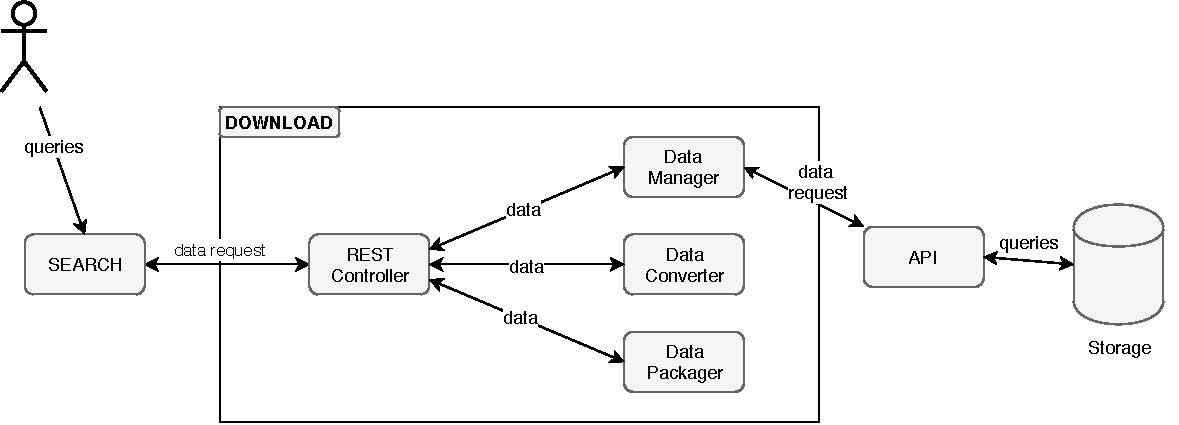
\includegraphics[width=\linewidth]{component.pdf}
\end{frame}
%------------------------------------------------
\begin{frame}
	\frametitle{Cross-cutting Requirements}
	\begin{center}
	\bgroup
	\def\arraystretch{1.5}
	% table generated online
	\begin{tabular}{|
		>{\columncolor[HTML]{9C27B0}}c |
		>{\columncolor[HTML]{7B1FA2}}c |
		>{\columncolor[HTML]{4A148C}}c |}
		\hline
		{\color[HTML]{FFFFFF} \begin{tabular}[c]{@{}c@{}}SEARCH\\ download button on UI
		\end{tabular}} & {\color[HTML]{FFFFFF} 
		\begin{tabular}[c]{@{}c@{}}DOWNLOAD\\ web server\end{tabular}} & 
		{\color[HTML]{FFFFFF} \begin{tabular}[c]{@{}c@{}}DATABASE\\ storage\end{tabular}} \\ \hline
	\end{tabular}
	\egroup
	\end{center}
	\begin{block}{}
		\begin{enumerate}
			\item \textbf{Performing a Download} search, download, database
			\item \textbf{Gathering Geospatial Data} download, database
		\end{enumerate}
	\end{block}
\end{frame}
%-------------------------------------------------
\begin{frame}
	\frametitle{Architectural Style: Three-tier}
	\begin{center}
		\bgroup
		\def\arraystretch{2}
		% generated table online, hence the mess 
		\begin{tabular}{|c|}
			\hline
			\rowcolor[HTML]{EF5350} 
			\multicolumn{1}{|c|}{\cellcolor[HTML]{EF5350}{\color[HTML]{FFFFFF} Client-server tier: Allows download server to handle requests}} \\ \hline
			\rowcolor[HTML]{E53935} 
			{\color[HTML]{FFFFFF} Business tier: converts and archives data} \\ \hline
			\rowcolor[HTML]{B71C1C} 
			{\color[HTML]{FFFFFF} Database-centric tier: requests geospatial data from database} \\ \hline
		\end{tabular}
		\egroup
	\end{center}
\end{frame}
%------------------------------------------------
\begin{frame}
	\frametitle{Frameworks}
	\begin{textblock*}{6cm}(5.5cm,3cm) % {block width} (coords)
		
\includegraphics[width=\textwidth]{express.png}
	\end{textblock*}
	\begin{textblock*}{6cm}(1cm,5cm) % {block width} (coords)
		
\includegraphics[width=\textwidth]{node.png}
	\end{textblock*}
\end{frame}
%------------------------------------------------
\begin{frame}
	\frametitle{Class Diagram}
	\begin{center}
		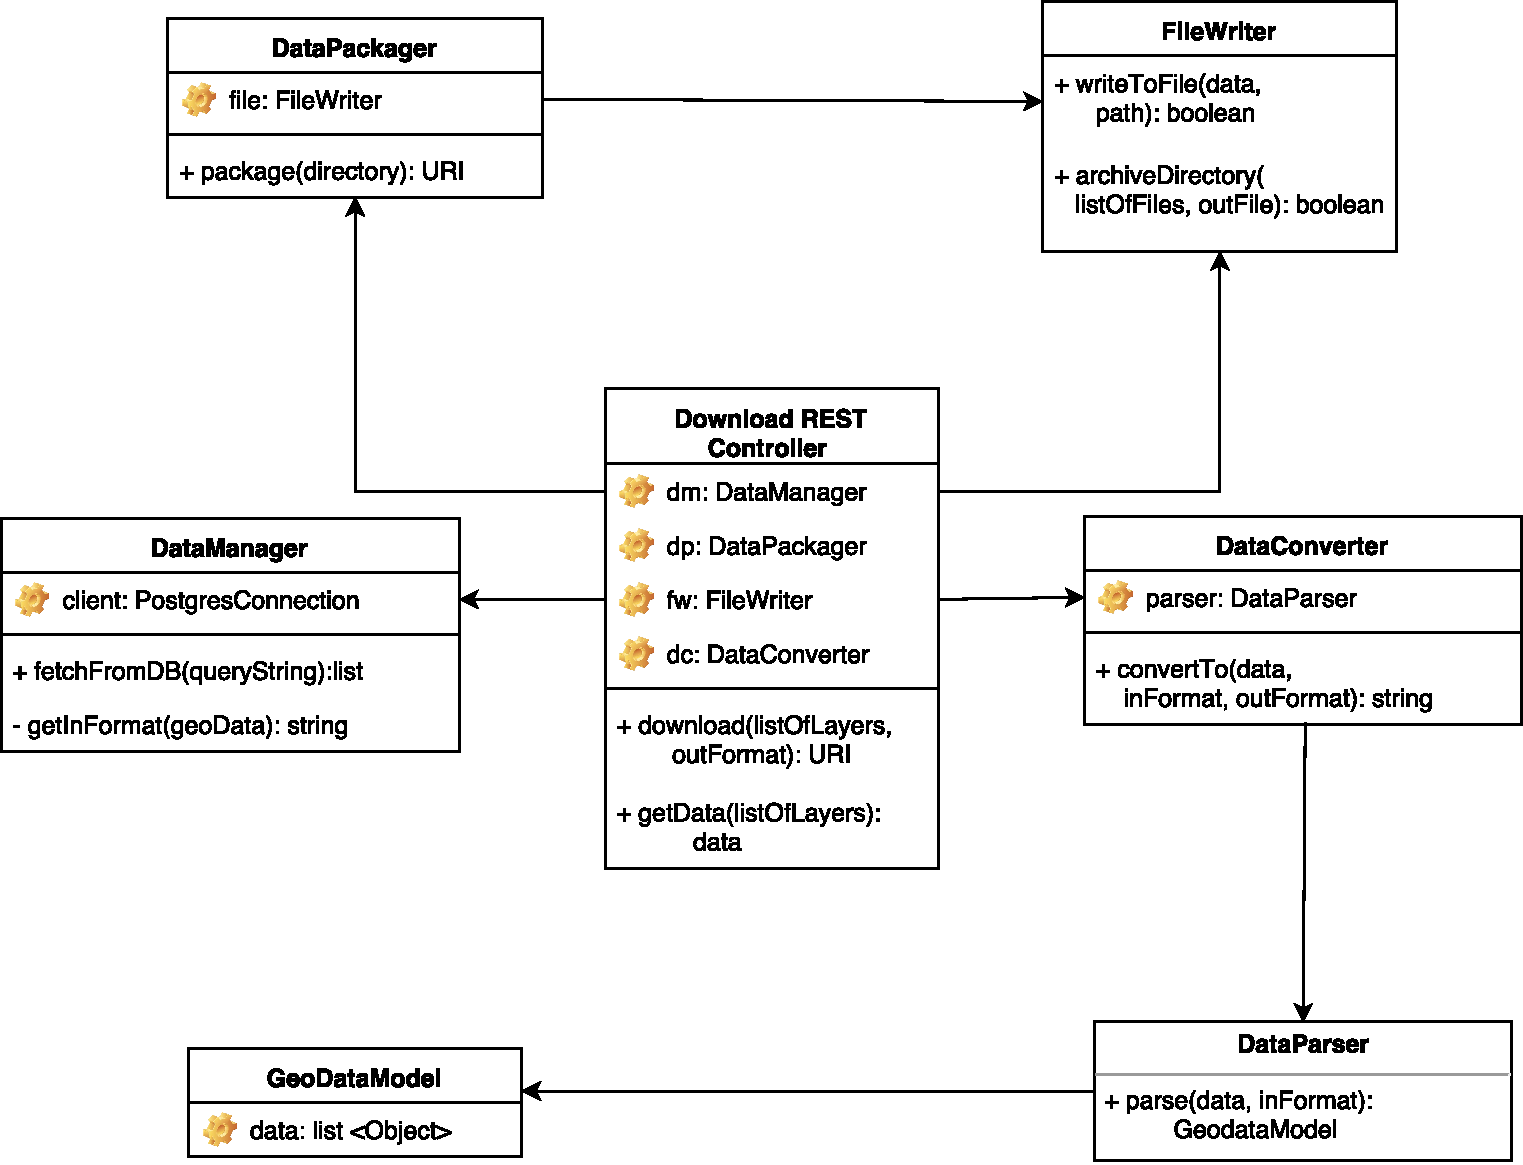
\includegraphics[width=0.8\linewidth]{class_diagram.pdf}
	\end{center}
\end{frame}
%-----------------------------------------------
\begin{frame}[plain]
	\frametitle{Sequence Diagram}
	\begin{center}
		\hspace*{-12mm}
		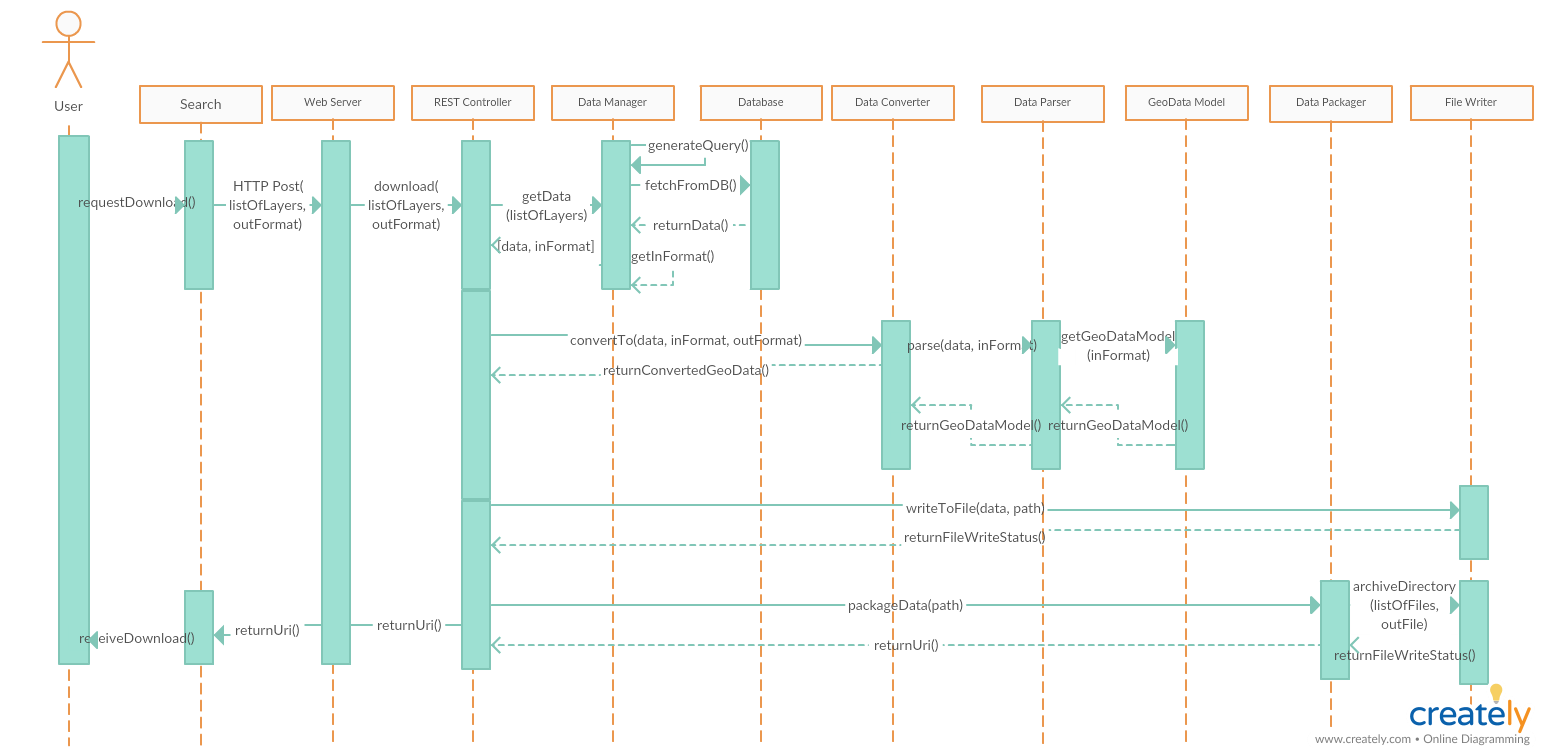
\includegraphics[width=\paperwidth]{download_sequence_diagram_v2.png}
	\end{center}
\end{frame}
%----------------------------------------------------
\begin{frame}
	\Huge{\centerline{Questions?}}
\end{frame}

\end{document}
